\chapter{基于PWF的极化SAR图像舰船目标检测}
\label{cha:PWF}

\section{引言}
\label{sec:intro}
在SAR图像中,斑点噪声是影响图像品质的主要因素之一。通常其由一个分辨单元内多个散射体的回波
相干叠加形成。相干斑的存在导致舰船目标检测中的虚警、漏报率提升,从而影响舰船目标检测的性能,
因此相干斑噪声的处理一直被认为是SAR图像处理中最重要的问题。在拥有多极化的SAR数据后,通过
将散射矩阵各个通道信息进行融合,提取极化特征,可以获取相干斑抑制的重构图像。通常图像SPAN即
散射总功率为最基本的极化特征,相较于单通道SAR图像,其可以显著的减少SAR图像中的相干斑噪声。在本章中
采用了重构图像的标准差s与均值m比进行相干斑噪声的衡量,并证明了极化白化滤波器可以使该比值达到最小,
从而得到最优的重构图像。最后我们采用PWF方法与恒虚警率检测器对极化SAR图像进行处理,结果表明基于极化白化
滤波器的CFAR方法可以有效鉴别海上舰船目标。

\section{海杂波统计特性}
    此章采用复高斯模型来描述海杂波的数学统计特性,包含三个通道的极化散射矢量描述如下
    \begin{equation}
      {\bf{X}}{\rm{ = }}\left[ {\begin{array}{*{20}{c}}
        {{{\bf{S}}_{hh}}} \\
        {{{\bf{S}}_{hv}}} \\
        {{{\bf{S}}_{vv}}} 
        \end{array}} \right]   
    \end{equation}
    极化散射矢量中的HH,HV,VV通道满足联合复高斯分布,因此极化散射矢量满足如下的概率密度分布
    \begin{equation}
        f({\bf{X}}) = \frac{1}{{{\Pi ^3}\left| {{\Sigma _c}} \right|}}\exp ( - {{\bf{X}}^H}\Sigma _c^{ - 1}{\bf{X}})
    \end{equation}
    其中${{\Sigma _c}}=E({\bf{X}}{{\bf{X}}^H})$是极化散射矢量的协方差矩阵,$H$代表共轭转置,${\rm{E}}( \cdot )$代表求期望。通常假设海杂波
    散射矢量的均值为零即$E({\bf{X}})=0$,当同极化矢量$ {{{\bf{S}}_{hh}}}$与交叉极化矢量${{{\bf{S}}_{hv}}}$间存在耦合时,海杂波散射矢量的极化协方差矩阵
    可以描述为以下的形式:
    \begin{equation}
        {\Sigma _c} = {\sigma _{hh}}\left[ {\begin{matrix}
   1 & 0 & {\rho \sqrt \gamma  }  \\ 
   0 & \varepsilon  & 0  \\ 
   {{\rho ^*}\sqrt \gamma  } & 0 & \gamma   \\ 
   \end{matrix}} \right]
    \end{equation}
    在上式中$*$代表共轭转置,符号变量的定义如\ref{equ:chap3:covdef}所示。

    \begin{equation}
        \label{equ:chap3:covdef}
        \begin{array}{l}
        {\sigma _{hh}} = E({\left| {S_{hh}} \right|^2})\\
        \varepsilon  = \frac{{E({{\left| {S_{hv}} \right|}^2})}}{{E({{\left| {S_{hh}} \right|}^2})}}\\
        \gamma  = \frac{{E({{\left| {S_{vv}} \right|}^2})}}{{E({{\left| {S_{hh}} \right|}^2})}}\\
        \rho  = \frac{{E(S_{hh} \cdot S_{vv})}}{{\sqrt {E({{\left| {S_{hh}} \right|}^2})E({{\left| {S_{vv}} \right|}^2})} }}
        \end{array}
    \end{equation}

\section{极化白化滤波器}
    利用HH,HV,VV三个通道的极化信息构建最优图像,采用重构图像的标准差$s$与均值$m$之比进行斑点噪声的度量。下面将
    证明极化白化滤波器可以使得重构图像的标准差与均值的比值达到最小。

    \begin{equation}
        \label{equ:chap3:measure}
        \frac{s}{m} = \frac{{\sigma (y)}}{{E(y)}}
    \end{equation}

    式\ref{equ:chap3:measure}中随机变量$y$代表重构图像的像素值,当给定SAR图像HH、HV、VV通道极化信息后,通过式\ref{equ:chap3:construct}来重建斑点
    抑制图像

    \begin{equation}
        \label{equ:chap3:construct}
        y = {{\bf{X}}^H}A{\bf{X}}
    \end{equation}
    在式\ref{equ:chap3:construct}中,权重矩阵A厄米共轭且正定,为了计算得到最优权重矩阵$A^*$,将式
    \ref{equ:chap3:measure}做式\ref{equ:chap3:trans}所示变换。式\ref{equ:chap3:trans}中,$\lambda_1, \lambda_2, \lambda_3$为
    矩阵${\Sigma _c}A$的特征值,因此寻找最优权重矩阵的问题被转化为寻找特征值$\lambda_1, \lambda_2, \lambda_3$
    使得$s/m$比值达到最小。显然当矩阵$\Sigma_cA$为单位阵、特征值$\lambda_1=\lambda_2=\lambda_3$时,该比值达到最小。
    因此$A^*$=$\Sigma_c^{-1}$被称作极化白化滤波器。


    \begin{equation}
        \label{equ:chap3:trans}
        \begin{array}{*{20}{c}}
            {\sigma (y) = tr{{({\Sigma _c}A)}^2} = \sqrt {\mathop \Sigma \limits_{i = 1}^3 {\lambda _i}^2} }\\
            {E(y) = tr({\Sigma _c}A) = \mathop \Sigma \limits_{i = 1}^3 {\lambda _i}}\\
            {\frac{s}{m} = \frac{{\sqrt {\mathop \Sigma \limits_{i = 1}^3 {\lambda _i}^2} }}{{\mathop \Sigma \limits_{i = 1}^3 {\lambda _i}}}}
        \end{array}
    \end{equation}

    获得极化白化滤波器后,通过式\ref{equ:chap3:recon}计算相干斑抑制的重构图像。从式\ref{equ:chap3:recon}
    可以看出相干斑抑制图像是对${{{\left| {{S_{hh}}} \right|}^2}}$,${{{\left| {{S_{hv}}} \right|}^2}}$,
    ${{{\left| {{S_{vv}}} \right|}^2}}$三个通道进行优化权重求和得到的强度图像。相较于单极化强度图像,极化白化
    滤波器提供了$4.8dB$的相干斑噪声抑制。

    \begin{equation}
        \label{equ:chap3:recon}
        y = \frac{{{{\left| {{S_{hh}}} \right|}^2}}}{{{\sigma _{hh}}(1 - {{\left| \rho  \right|}^2})}} + \frac{{{{\left| {{S_{vv}}} \right|}^2}}}{{{\sigma _{hh}}(1 - {{\left| \rho  \right|}^2})\gamma }} + \frac{{{{\left| {{S_{hv}}} \right|}^2}}}{{{\sigma _{hh}}\varepsilon }} - \frac{{2{\mathop{\rm Re}\nolimits} (\rho  \cdot {S_{hh}}^* \cdot {S_{vv}})}}{{{\sigma _{hh}}(1 - {{\left| \rho  \right|}^2})\sqrt \gamma  }}
    \end{equation}

   采用实验数据来验证PWF相干斑抑制效果,实验数据选择的是C波段多极化大连港的原始SAR图像数据,所截取的图像为1000x1000的
   海洋场景,在自适应极化白化滤波器方法中,使用大小为31x31的滑动窗选择海杂波像素来计算极化白化滤波器参数,下表为原图像HH通道、SPAN方法与APWF
   (自适应极化白化滤波器)方法处理后图像的标准差与均值比。

  \begin{table}[htb]
  \centering
    \begin{minipage}[t]{0.8\linewidth} % 如果想在表格中使用脚注,minipage是个不错的办法
    \caption[不同强度图像s/m比值]{HH、SPAN与APWF强度图像标准差与均值比}
    \label{tab:template-files}
      \begin{tabularx}{\linewidth}{lXXX}
        \toprule[1.5pt]
        {\heiti 滤波方法} & {\heiti HH强度图像} & {\heiti SPAN强度图像} & {\heiti APWF强度图像}\\ \midrule[1pt]
        s/m & 2.02 & 2.25 & 11.24 \\
        \bottomrule[1.5pt]
      \end{tabularx}
    \end{minipage}
\end{table}

  从不同强度图像结果中可以看到,SPAN强度图像与APWF强度图像对相干斑都有抑制效果,并且增强了船-海之间的对比对,可以对重构强度图像进行统计
  分析来进一步实施舰船检测~\cite{Novak1989Optimal}。

 \section{自适应PWF舰船检测算法}
不同天气条件下的海况不同,因此在SAR图像不同区域的杂波表现差别也很大,为了让算法具有更好的普适性,
采用自适应极化白化滤波器(Adaptive PWF)舰船检测方法。本章前三节描述了当海杂波散射矢量满足复高斯分布时,
可以采用滑动窗选择局部海杂波散射矢量计算极化白化滤波器参数,并使用该滤波器生成相干斑抑制图像,在文献~\cite{J1986Speckle}
中表明,使用自适应极化白化滤波器生成的重构强度图像值满足如下分布:

\begin{equation}
  \label{equ:chap3:pdf}
  {f_y}(y) = {(N)^{N - \rho  + 1}}\frac{{{y^{(\rho  - 1)}}}}{{{{(y + N)}^{N + 1}}}}\frac{{\Gamma (N + 1)}}{{\Gamma (\rho )\Gamma (N - \rho  + 1)}}
\end{equation}
式\ref{equ:chap3:pdf}中,$\rho$为极化散射矢量的维度,$N$为滑动窗内极化散射矢量的个数。当给定恒虚警率
时依据式\ref{equ:chap3:pdf}我们可以计算检测阈值,当$N$很大时检测阈值与恒虚警率近似有式\ref{equ:chap3:threshold}所示的关系。式\ref{equ:chap3:threshold}中,$T$代表
检测阈值,$P_{FA}$为恒虚警率。

\begin{equation}
  \label{equ:chap3:threshold}
  {P_{FA}} = \exp ( - T)\mathop \Sigma \limits_{k = 0}^{\rho  - 1} \frac{{{T^k}}}{{k!}}
\end{equation}

整个算法流程如Alogrithm~\ref{alg:chap3:APWF}所示,在该算法中要对图像中的所有像素值进行判断,
因此使用的滑动窗的个数等于图像的像素数量。对于大小为N\times N的滑动窗,计算滑动窗对应的滤波器参数的算法时间复杂度为$O(N^2)$,
整个算法的时间复杂度为$O(mnN^2)$,m、n为SAR图像的宽度与高度,因此基于APWF检测算法的运行时间与滑动窗和原始SAR图像大小有关。当图像或滑动窗尺寸较大
时,算法的时效性差不能满足实时检测的要求,所以要在时间方面进行优化。在AWPF算法中,各个滑动窗所对应的自适应极化
白化滤波器参数估计相互独立,因此可以采用并行计算的方式来提高算法的运行效率。

\begin{algorithm}[t]
  \caption{自适应极化白化滤波器舰船检测算法}
  \label{alg:chap3:APWF}
	\KwIn{极化SAR数据,$S_{hh}$,$S_{hv}$,$S_{vv}$}
  \BlankLine
  
  对原始图像边缘根据所选择的滑动窗大小做镜像延拓。

	\ForEach{图像中的像素}{
      从原始SAR图像中根据滑动窗选择海杂波散射矢量$\bf{X}$

      计算自适应极化白化滤波器参数

      根据自适应极化白化滤波器生成重构强度图像值$y$

      依据式\ref{equ:chap3:threshold},采用牛顿迭代法得到检测阈值$T$

      得到检测结果$result = y > T$
	}
  \KwOut{二值舰船检测结果图像$result$}  
 \end{algorithm}

\section{基于GPU的PWF算法实现}

\subsection{GPU算法设计与优化}
 对于APWF舰船检测方法,不同像素对应的自适应极化白化滤波器参数计算过程完全相同,只是通过滑动窗
 选取的海杂波数据不同,因此我们将可并行且计算密集的滤波器参数计算部分放到GPU上去执行如算法\ref{alg:chap3:APWFCUDA}所示。在GPU编程模型中
 ,线程有两个并行的层次分别是网格层次和线程块层次,一个线程块中的线程会作为一个整体被调度到流多处理器上
 去执行。为充分利用GPU硬件资源,将线程块大小设计为32x32即每个线程块中包含1024个线程,网格大小设计为16x16。
 实验中使用的图像大小为1000x1000,故让一个线程块中共1024个线程对应处理SAR图像一行的数据,每个线程通过自身的
 二维索引和SAR图像中的像素一一对应。

 将线程索引与像素索引对应后,从GPU全局内存(Global Memory)中读取该像素对应滑动窗所选的海杂波数据。在一个线程块内,数据的读取是以线程束的方式进行的。
 一个线程束中包含32个线程,当线程束中线程访问的数据地址在128字节范围内时,该访问可以进行合并。合并访问可以大大
 加快内存访问的速度,提升总线利用效率。因此在算法设计过程中,将全局数据复制到线程私有空间采用按行访问的形式可以保证
 线程束中线程访问的地址空间位于128字节范围内。

  \begin{figure}[H] % use float package if you want it here
    \centering
    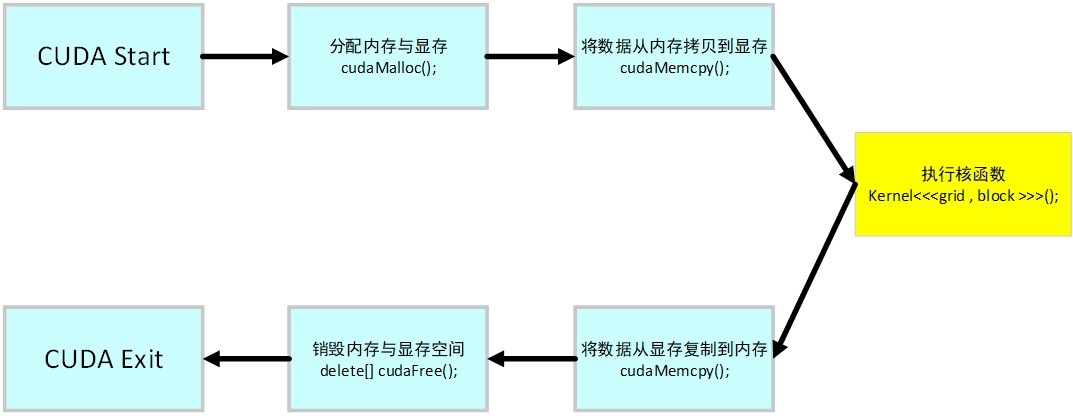
\includegraphics[width=0.8\textwidth]{kernel.jpg}
    \caption{CUDA执行流程}
    \label{fig:chap3:kernel}
  \end{figure}

\begin{algorithm}[t]
  \caption{并行PWF方法CUDA简化执行流程代码}
  \label{alg:chap3:APWFCUDA}

  cudaSetDevice();\\cudaMemcpy2D(imgGPU, pitch imgCPU, pitch, size, n cudaMemcptHostToDEvice);

  cudaStreamCreate(Stream1)

  fPWF< < <grid,block,0,stream1> > >(parameters)

  cudaDeviceSynchronize()

  cudaMemcpy(resCPU,resGPU,size,cudaMemcpyDeviceToHost)

  imshow(); Timeshow()

 \end{algorithm}
 核函数的设计,在GPU上所有的线程按照单指令多线程的方式去执行。不同的线程在其私有数据空间上去执行相同的指令。对于APWF
 方法,核函数的主要任务是计算极化白化滤波器参数即海杂波散射矢量的协方差矩阵的逆,协方差矩阵计算主要涉及一个3\times N与一个N\times 3
 的矩阵相乘,对于该矩阵乘法,采用了动态并行的方式进行了进一步的优化,从当前核函数中创建新的核函数来完成矩阵并行乘法运算。
 得到滤波器参数后,按照式\ref{equ:chap3:construct}生成重构强度值,并与牛顿迭代法获得的阈值做分割,输出二值检测结果
 图像。
\subsection{多GPU协同算法设计}

 多GPU协同APWF方法实现,当多个GPU通过PCIe总线连接时,不同GPU设备之间可以进行通信与同步。多GPU编程中要首先确定
 系统中可用的GPU数量,之后将计算任务合理的分配到各个GPU上。在APWF算法设计中,首先为各个GPU设备分配设备内存,流和事件
 并将SAR图像数据从主机内存拷贝至设备内存。然后依据系统的GPU数量,将原SAR图像进行按行划分并将计算任务分配到不同的GPU流上。
 当流中的核函数执行完成后,将不同GPU上的检测结果复制到主机内存中,作为最终的检测结果。在多GPU编程实现过程中,为了便于
 多GPU之间进行通信,采用了统一虚拟寻址的技术,将所有变量映射到相同的虚拟地址空间中,方便主机和设备进行访问。

 \section{实验结果与加速比测试}

 本次实验在NVDIA TIATN V平台上对APWF舰船检测方法进行测试,图\ref{fig:chap3:resultPWF}为海洋SAR图像检测结果,为了
 衡量SAR图像的检测效果,定义$F_1=\frac{{{N_{tt}}}}{{{N_{fa}} + {N_{gt}}}}$作为评价指标,其中$N_{tt}$为正确检测舰船目标个数,$N_{fa}$
 为虚警的数量,$N_{gt}$为数据船只的真实数量。

 本次实验采用的GPU平台为NVIDIA TiTan V, 相对比的CPU平台为(Intel(R) Core(TM) i9-7920X CPU)处理器,实验所用SAR图像大小为1000\times 1000
 ,滑动的大小为31\times 31。经过多次测试,不同算法消耗时间如表\ref{tab:chap3:PWFtimeresult}所示。由测试结果可知基于GPU的多线程PWF检测方法
 在检测效率上提升了近32倍,而基于多GPU协同的PWF方法在双GPU的条件下检测时间性能提升了53倍。


  \begin{figure}[h]
    \centering
    \subcaptionbox{SPAN图\label{fig:subfig2}}
        {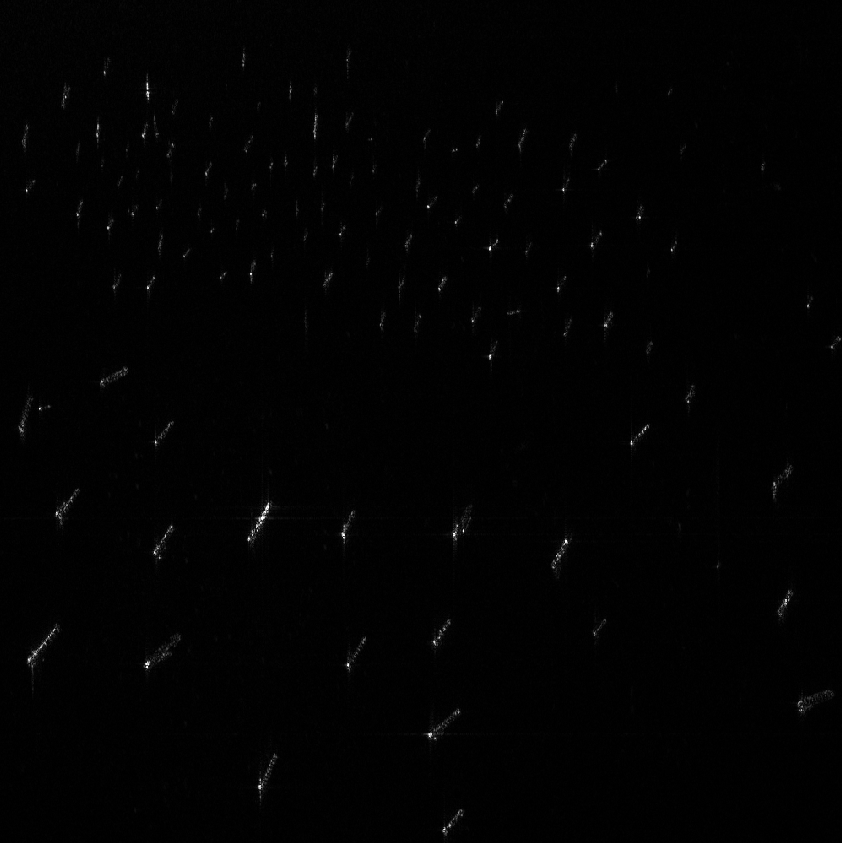
\includegraphics[width=5cm]{HHSPAN.png}}
    \subcaptionbox{PWF检测结果\label{fig:subfig2}}
        {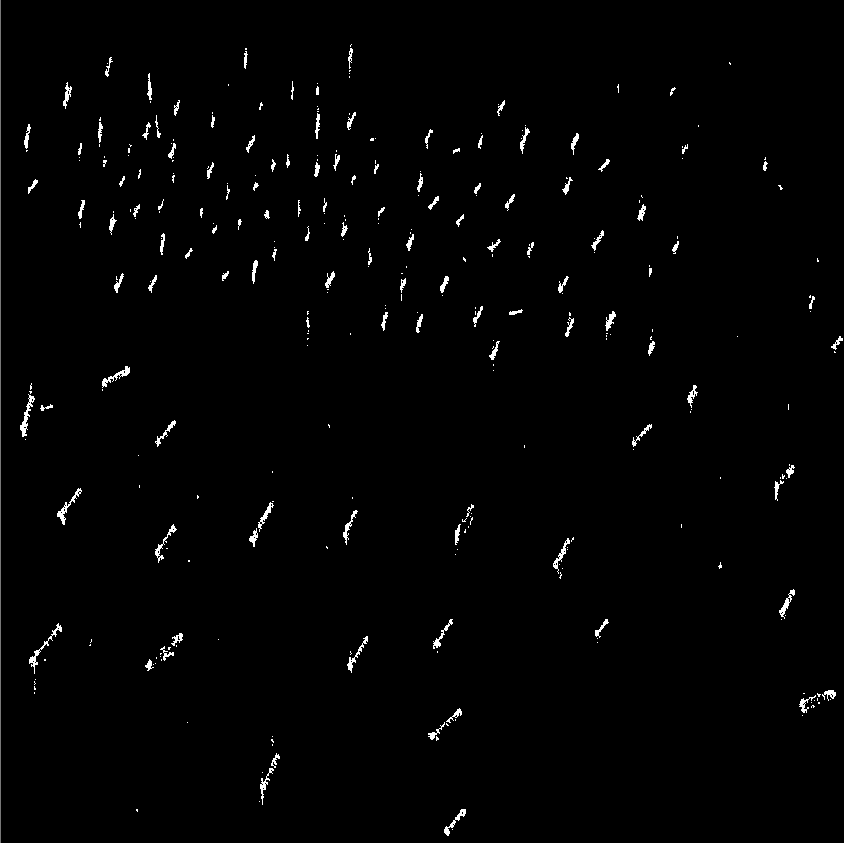
\includegraphics[width=5cm]{resultPWF.png}}
    \caption{PWF图像检测结果}
    \label{fig:chap3:resultPWF}
  \end{figure}

  \begin{table}[htb]
  \centering
    \begin{minipage}[t]{1\linewidth} % 如果想在表格中使用脚注,minipage是个不错的办法
    \caption[Adaptive PWF检测结果]{SAR图像极化白化滤波器检测结果}
    \label{tab:chap3:detectresult}
      \begin{tabularx}{\linewidth}{lXXXXXX}
        \toprule[1.5pt]
        {\heiti 检测方法} & {\heiti 船只总数} & {\heiti 总检测数量} & {\heiti 正确检测数量} & {\heiti 虚警数量} & {\heiti 漏报数量} & {\heiti $F_1$}\\ \midrule[1pt]
        PWF & 118 & 123 & 117 & 6 & 1 & 0.943\\
        \bottomrule[1.5pt]
      \end{tabularx}
    \end{minipage}
\end{table}

  \begin{table}[htb]
  \centering
    \begin{minipage}[t]{1\linewidth} % 如果想在表格中使用脚注,minipage是个不错的办法
    \caption[PWF不同平台运行时间]{不同平台PWF算法运行时间}
    \label{tab:chap3:PWFtimeresult}
      \begin{tabularx}{\linewidth}{lXX}
        \toprule[1.5pt]
      {\heiti 检测算法} & {\heiti 运行平台} & {\heiti 运行时间/s} \\ \midrule[1pt]
        PWF(C++) & (Intel(R) i9-7920X CPU) & 67.4\\
        GPU多线程PWF &  GPU(Titan V) & 2.1 \\
        多卡协同PWF & 2 GPU(Titan V) & 1.27 \\
        \bottomrule[1.5pt]
      \end{tabularx}
    \end{minipage}
\end{table}

\section{小结}
  在本章中,我实现了基于GPU的高性能并行极化白化滤波器SAR图像舰船目标检测算法。本章首先对
  自适应极化白化滤波器检测算法原理进行分析,然后结合GPU架构特点,将计算密集且可并行的滤波器参数计算部分
  放到GPU上去并行执行,并进一步将数据和计算任务分配到多GPU上去执行,对原算法在时间性能上进行优化。实验结果表明,
  相比于串行基于CPU的检测方法,基于GPU的并行检测算法在时间性能上获得了数十倍的提升。


